% Chapter 9 -- translated by Claude (2026), continuing the voice and
% register of the Burkett-Hutcheson chapters.

\chapter{Some new concepts}

\section{Problems with graphs}

Sometimes it is necessary to build a graph with the answers. There
are, basically, four types of graphs related to a Symbulator
simulation:

\begin{enumerate}
\item The value of an answer obtained in an AC analysis, as a
  function of the frequency $\omega$.
\item The value of an answer obtained in an FD analysis, as a
  function of the complex frequency $s$.
\item The value of an answer obtained in a TR analysis, as a
  function of time $t$.
\item The value of any answer, as a function of a symbolic circuit
  value.
\end{enumerate}

Your calculator has extensive graphing capabilities. The detailed
description of their diversity and use is beyond the purpose of this
book; however, it is available in the User's Manual of the
calculator.

In Chapter 12 we will see an example of the second type of graph
using the \code{bode} tool, and an example of the third type of
graph, using the \code{plot} tool.

Next, we will see an example of the first type of graph, using the
calculator's own capabilities. The technique that will be shown is
also applicable to the fourth type of graph.

\problem{064}

\emph{Problem: Graph $\mathrm{abs}(V_{out})$ against $\omega$ for
the circuit shown in the figure. Cover a frequency interval from
$\omega = 800$ to $\omega = 1200$~rad/s.}


% figures added 10 Sep 2026
\begin{figure}[!ht]
\centering
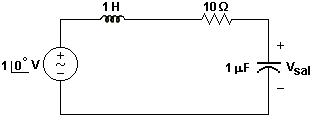
\includegraphics[width=106mm]{book_figures/p064_0.png}
\caption*{Circuit for Problem 064}
\end{figure}

Solution: We will simply use the simulation and the graphing
capabilities of the calculator:

\begin{entry}
sq\ac("e,1,0,1;l,1,2,1;r,2,3,10;c,3,0,1E-6",x)
\end{entry}

A frequency \code{x} was used with the intention that the output
voltage remain a function of the variable \code{x}. The purpose of
this is to satisfy the requirement of the calculator, which demands
that the functions \code{y\#} to be graphed, where \# is a number,
be given as functions of \code{x}, where \code{x} is the independent
variable.

We press \key{ENTER}. The simulation takes some time. Finally `Done'
appears. The next step is to make the value of
$\mathrm{abs}(V_{out})$ appear in the history area. We can use
either \code{v3} or \code{vc} as $V_{out}$:

\begin{entry}
abs(v3)
\end{entry}

We press \key{ENTER}. We obtain a function of \code{x}, which we
will store in any of the functions \code{y\#(x)}, where \# is a
number:

\begin{entry}
ans(1)→y1(x)
\end{entry}

We press \key{ENTER} and the function is stored in the specified
variable. Pressing \key{$\diamond$} \key{Y=} we can verify that this
is so. Now we can specify the range of frequencies for which we wish
to graph. We press \key{$\diamond$} \key{WINDOW} and specify for
\code{xmin} a value of 800 and for \code{xmax} a value of 1200. We
press \key{$\diamond$} \key{GRAPH} and see the graph. We can press
\key{F2} \key{A} on the TI-89 to apply the ZoomFit command, which
adjusts the height of the graph to the best value.

We have learned how to graph an answer as a function of frequency,
using the calculator's own capabilities.

\section{Problems with multiple unknowns}

To solve a circuit with symbolic values, we need to have one answer
known in advance for each symbolic value whose numerical value is
unknown and desired. To solve a system, we require the same number
of equations as unknowns. We will see a problem in which both axioms
are satisfied at the same time, but first, a theoretical
clarification. We explained in Chapter 7 that before simulating a
circuit containing a two-port, we must have stored in memory the
values of the four parameters of that two-port, under the
corresponding names. But what happens if we do not store these
values? Symbulator will simulate the circuit using the parameters
that are not stored before the simulation as if they were symbolic
variables.

\problem{065}

\emph{Problem: Complete the given table, and also give the values of
the $y$ parameters.}


% figures added 10 Sep 2026
\begin{figure}[!ht]
\centering
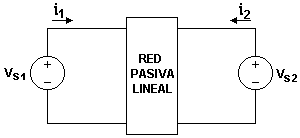
\includegraphics[width=102mm]{book_figures/p065_0.png}
\caption*{Circuit for Problem 065}
\end{figure}

Solution:

This is a very special problem, which allows us to enjoy the
symbolic capabilities of Symbulator. There are several ways to solve
it. Here we will present the most linear and simple way, which
however is not the most sophisticated.

Although the problem statement presents the two questions in that
order, to answer them we will invert them. That is, first we will
find the values of the $y$ parameters, and then we will complete the
table. To find the $y$ parameters, we will take advantage of the
first two rows of the table, which are already complete. It is
precisely thanks to these complete rows that we will be able to
generate the four equations necessary to find the four numerical
values of the parameters \code{yp11}, \code{yp12}, \code{yp21} and
\code{yp22}. The steps we will follow are these:

\begin{enumerate}
\item Simulate the circuit, without defined parameters.
\item Use the two complete rows of the table to generate the four
  equations we need.
\item Obtain the four numerical values of the parameters, solving
  these four equations.
\item Complete the table, using the parameters we have found and the
  values given by the incomplete rows.
\end{enumerate}

The procedure is as follows:

\begin{entry}
sq\dc("j1,0,1,j1;j2,0,2,j2;yp,1,2,0")
\end{entry}

We press \key{ENTER}. The simulation runs and `Done' appears. We
generate the first equation with the following command:

\begin{entry}
v1=100|j1=5 and j2=-32.5
\end{entry}

With \key{ENTER} we obtain the equation. We generate the second
equation like this:

\begin{entry}
v2=50|j1=5 and j2=-32.5
\end{entry}

With \key{ENTER} we obtain the equation. We generate the third
equation like this:

\begin{entry}
v1=50|j1=-20 and j2=-5
\end{entry}

With \key{ENTER} we obtain the equation. We generate the fourth
equation like this:

\begin{entry}
v2=100|j1=-20 and j2=-5
\end{entry}

Having generated the four equations, we proceed to solve them to
find the four $y$ parameters:

\begin{entry}
solve(ans(1) and ans(2) and ans(3) and ans(4),
      {yp11,yp12,yp21,yp22})
\end{entry}

With \key{ENTER} we obtain the parameters: \code{yp11}~$= .2$ and
\code{yp12}~$= -.3$ and \code{yp21}~$= -.4$ and
\code{yp22}~$= .15$. Now, we proceed to complete the table. To
complete the third row, we use the following command:

\begin{entry}
solve(v1=20 and v2=0,{j1,j2})|ans(1)
\end{entry}

With \key{ENTER} we obtain the missing values in the row:
\code{j1}~$= 4.$ and \code{j2}~$= -8.$ To complete the fourth row,
we use the following commands:

\begin{entry}
v1|ans(2) and j1=5 and j2=0
v2|ans(3) and j1=5 and j2=0
\end{entry}

Note how the number \# that appears in \code{ans(\#)} changes to
reflect, at each moment, the new position of the answers holding the
$y$ parameters. With \key{ENTER} we obtain the values $-8.33333$ and
$-22.22222$, respectively. To complete the fifth row, we use the
following commands:

\begin{entry}
v1|ans(4) and j1=5 and j2=15
v2|ans(5) and j1=5 and j2=15
\end{entry}

With \key{ENTER} we obtain the values $-58.33333$ and $-55.55555$,
respectively. So, we have completed the table.

Personally, I consider this one of the most interesting problems I
have ever solved, using Symbulator.

Let us learn to use a new element.

\section{The ideal operational amplifier (ideal op-amp)}

An ideal op-amp is, in essence, a voltage-dependent voltage source.
By saying it is ideal, we mean that its parameters are considered as
$R_i = \infty$, $R_o = 0$ and $A = \infty$.

\subsection{Notation}

In the case of the ideal op-amp, the minimum information necessary
to describe it completely is the following:

\emph{Identification.} The letter that identifies an ideal op-amp is
\code{o}.

\emph{Name.} It must be given any name that begins with the letter
\code{o}.

\emph{Nodes.} An ideal op-amp, as Symbulator understands it, has
three connection points: one positive, one negative and one output.

So, ideal op-amps are defined as shown below:

\begin{entry}
oname, node +, node -, output node
\end{entry}

The description of the ideal op-amp always has 4 terms, so there
could be a need to add a zero at the end.

\subsection{Related answers}

In the case of an ideal op-amp, one related answer is given: the
current that leaves the op-amp through the output node. This current
is stored in a variable called \code{iname}, where \code{name} is
the name of the ideal op-amp. So, for an ideal op-amp called
\code{o1}, the related answer will be \code{io1}. Remember that this
current is considered as leaving the op-amp.

Let us see some examples.

\problem{066}

\emph{Problem: Given the following circuit, find the voltage at the
output node of the ideal op-amp.}


% figures added 10 Sep 2026
\begin{figure}[!ht]
\centering
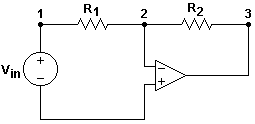
\includegraphics[width=87mm]{book_figures/p066_0.png}
\caption*{Circuit for Problem 066}
\end{figure}

Solution: After clearing the symbolic variables we are going to use,
we order the simulation, and request the voltage at the output node
of the op-amp:

\begin{entry}
DelVar r1,r2,vin:sq\dc("e1,1,0,vin;r1,1,2,r1;r2,2,3,r2;
o1,0,2,3"):v3
\end{entry}

With \key{ENTER}, the simulation starts and we obtain the answer:
\code{-r2*vin/r1}.

\problem{067}

\emph{Problem: If the op-amp shown is assumed ideal, find
$R_{in}$.}


% figures added 10 Sep 2026
\begin{figure}[!ht]
\centering
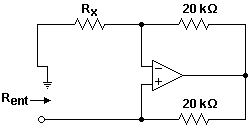
\includegraphics[width=85mm]{book_figures/p067_0.png}
\caption*{Circuit for Problem 067}
\end{figure}

Solution: Let us use the \code{thevenin} tool:

\begin{entry}
DelVar rx:sq\thevenin("rx,1,0,rx;r1,1,2,2E4;r2,2,3,2E4;
o1,3,1,2",3,0)
\end{entry}

With \key{ENTER}, the tool executes. We choose Passive and DC. We
press \key{ENTER}. We obtain the answer on the screen (and in
memory): \code{zth}~$=$~\code{-rx}.

These examples illustrate the ease with which ideal op-amps are
simulated in Symbulator.

\section{Final considerations for the (Expert) Mode}

This section should be read by those users who have already read
Chapter 4.

\subsection{Restrictions of the (Expert) Mode with op-amps}

As we have said, the (Expert) Mode allows the user to choose whether
to solve the equations, solve and keep them, or simply keep them.
Circuits containing ideal operational amplifiers will generate
equations that are not comprehensible to the user, because they
contain a term that will later be used for the application of the
calculator's limit command. Therefore, when the circuit solved in
the (Expert) Mode includes op-amps, you must always choose
Symbulate, and never Just Keep, when the dialog asks for the
procedure you wish to follow.

\subsection{Restrictions of the (Expert) Mode in transient
analysis}

In Chapter 10 we will learn to run simulations in the frequency
domain (FD). In Chapter 11 we will learn to run transient analysis
(TR) simulations. During a transient analysis, the simulator will
generate equations in the frequency domain. After solving these
equations, all the answers are converted to the time domain.
Therefore, when the simulation in the (Expert) Mode is a transient
analysis, we must always choose Symbulate, and never Just Keep, if
we wish to obtain answers in the time domain. Keeping the generated
equations and solving them later would lead us to answers in the
frequency domain.

\subsection{More first-level variables}

Some circuit elements were presented after Chapter 4. Let us learn
which of them have first-level variables related to them.

\emph{Inductors.} The current through them is a first-level
variable. Their voltage drop is a second-level variable that is not
replaced by its value at the end of the simulation. Their power is a
third-level variable.

\emph{Capacitors.} The current through them is a second-level
variable that is indeed replaced by its value at the end of the
simulation. Their voltage drop is a second-level variable that is
not replaced by its value at the end of the simulation. Their power
is a third-level variable.

\emph{Ideal transformers.} The current entering the transformer on
the primary side is a first-level variable. The current entering the
transformer on the secondary side is a second-level variable that is
not replaced by its value at the end of the simulation.

\emph{Two-ports.} The currents entering the two-port at both ends
are first-level variables.

\emph{Ideal operational amplifiers.} The current leaving the op-amp
through the output node is a first-level variable.
